\documentclass{article}
\usepackage[T1]{fontenc}
\usepackage[francais]{babel}
\usepackage[utf8]{inputenc}

\usepackage{amsmath,amsfonts,amsthm} % Math packages
\usepackage[pdftex]{graphicx}
\usepackage[hidelinks]{hyperref}
\usepackage{lipsum}

\usepackage{listings}
\usepackage{charter}
\usepackage{array}
\usepackage{here}
\usepackage[justification=centering,singlelinecheck=false]{caption}
\usepackage{subcaption}
\newcolumntype{M}[1]{>{\raggedright}m{#1}}
\newcommand{\HRule}{\rule{\linewidth}{0.5mm}}

\usepackage{color}
\definecolor{dkgreen}{rgb}{0,0.6,0}
\definecolor{gray}{rgb}{0.5,0.5,0.5}
\definecolor{mauve}{rgb}{0.58,0,0.82}

\begin{document}
\begin{titlepage}
\begin{center}

% Upper part of the page. The '~' is needed because \\
% only works if a paragraph has started.

\includegraphics[width=0.5\textwidth]{pictures/ul.png}~\\[1cm]

% Title
\HRule \\[0.2cm]
{ \huge \bfseries Simulation à base d'agents de l'évolution d'un
  logiciel Open Source \\[0.4cm] }

\HRule \\[1.5cm]
Quentin BAILLEUL \  Romain PHILIPPON

\vfill

% Bottom of the page
{\large \today}

\end{center}
\end{titlepage}

\newpage
\tableofcontents

\newpage

\section{Introduction}
%inspiration du abstract de base
L'informatique est une discipline qui évolue rapidement et
il est nécessaire de comprendre
les processus évolutifs qui prévalent dans de nouvelles formes de
développement de logiciels notamment dans un environement Open source.
\\

Beaucoup de travaux et d'analyses sont fournies à propos de la
création et de l'évolution de logiciels propriétaires, à l'inverse de
l'étude sur les logiciels Open Sources. 
\\

Ceci suggère que les théories existantes sur l'évolution des logiciels
sont différentes pour les logiciels open source.

Dans cette optique les recherches de N Smith, A Capiluppi, et
J Fernandez-Ramil tendent à améliorer voir redéfinir ces théories.
\\

Leur article utilise les théories de l'évolution du logiciel
afin de reproduire et d'expliquer les observations empiriques d'un ensemble
de systèmes Open Source. Pour cela, l'article se repose sur une simulation multi-agents de
développement logiciel dans un environement Open Source.
\\

Le but de ce rapport sera de modifier la simulation en ajoutant des
paramètres afin de rajouter du réalisme afin de comparer les résultats pour
déterminer si les règles du comportement suivent la règle du Rasoir d'Ocam, c'est à dire
qu'il suffit d'un ensemble de règles réduits au strict minimum pour reproduire l'évolution du
développement d'un logiciel open-source. Ou au contraire, si les résultats mis en lumière dans
ce rapport tendent à prouver l'inverse.
\\

Dans un premier temps, nous présenterons le modèle de N. Smith, A. Capiluppi et J. Fernandez-Ramil,
puis dans une seconde partie s'attardera sur la version modifiée et les nouveautés implémentées. Puis
dans la troisième partie, nous comparerons les résultats obtenus avec les résultats du modèle de base.
Puis nous terminerons par une conclusion.

\newpage

\section{Simulation de base}

\begin{figure}[H]
 \centerline{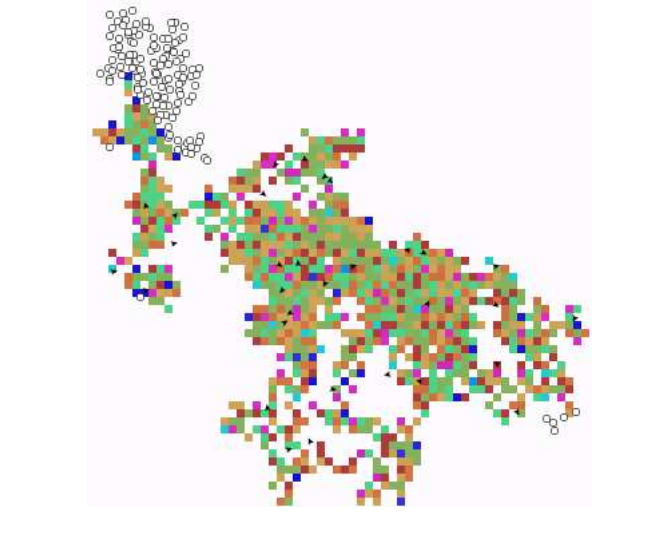
\includegraphics[scale=0.45]{pictures/Image0.png}}
\caption{Un exemple de développement de logiciel Open Source
  simulé. Les carrés sont des patches de code. Les cercles noirs
  sont des prérequis non satisfaits.}
 \end{figure}

La simulation du projet de N Smith, A Capiluppi, et J Fernandez-Ramil est basée sur trois types d'agents :

\subsection{Les Modules}
Un module représente une fonctionnalité du logiciel. Chaque module comporte un score de complexité et un score de santé (c'est-à-dire la stabilité du code). Ces scores varient selon l'action effectuée par le développeur. Un module peut créer des agents \textit{prérequis} si ses voisins (voisinage de Moore de 1) ne sont pas des modules.

\newpage

\subsection{Les Prérequis}
Les prérequis symbolisent une spécification logicielle qui attend qu'un module soit crée par développeur.

\subsection{Les Développeurs}
Un développeur se définit par son score d'ennui. Les développeurs se promènent aléatoirement dans l'espace de simulation. À chaque déplacement un développeur peut effectuer une des actions suivantes :

\begin{enumerate}
  \item Si il rencontre un prérequis le développeur produit à l'emplacement de celui-ci un module. Le prérequis meurt à l'issue de cette opération.
  \item{Si il se trouve sur un module et que la santé et la complexité ne dépasse pas un seuil donné, le développeur factorise le module. Cela induit une réduction de la complexité de ce dernier.}
  \item{Si il se trouve sur un module et qu'il ne peut pas le factoriser, il va le développer. C'est-à-dire qu'il augmente la complexité et la santé si et seulement si la complexité de ce module ne dépasse pas un seuil donné}
  \item{Si il ne peut pas réaliser une des actions présentées ci-dessus alors il incrémente son score d'ennui de 1}
\end{enumerate}

Dès que le développeur achève l'une de ces actions, il meurt si son score d'ennui est supérieur à un seuil. Sinon il se déplace en se dirigeant dans une direction aléatoire.

\section{Simulation modifiée}

\begin{figure}[H]
 \centerline{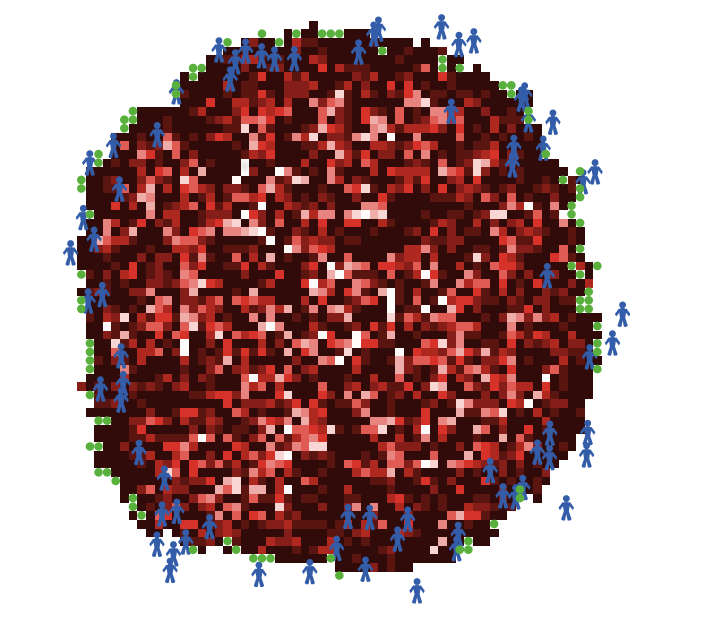
\includegraphics[scale=0.45]{pictures/Image1.png}}
\caption{Un exemple de développement de logiciel Open Source
  simulé via le modèle présenté dans ce papier.}
 \end{figure}

Pour apporter du réalisme à la simulation, plusieurs paramètres ont été introduits :

\subsection{Module}
Un module est maintenant déterminé par un langage de programmation. Il ne peut pas être développé ou factorisé si par un développeur ne connait pas ce langage. En outres, le module a aussi une chance d'être déstabilisé par le développeur (sa santé baissera) proportionnellement à son expérience. Plus un développeur est expérimenté moins il aura de chance de déstabiliser le code. Et quand bien même un développeur expérimenté introduit du code néfaste il ne sera pas aussi instable qu'un code introduit par un développeur inexpérimenté.

\newpage
\subsection{Développeur}
Un développeur est maintenant doté d'une expérience. Plus il développe ou factorise du code, plus son expérience augmente. L'expérience détermine la capacité plus ou moins importante à modifier le code (modification de la santé et/ou de la complexité du code). 
D'ailleurs, un développeur n'est plus en mesure de développer un module si celui-ci contient des \textit{prérequis} dans son entourage. Le but est de modéliser les dépendances entre modules.
\\

Le développeur est aussi doté d'une panoplie de langages connus qui lui permet de travailler sur les modules dont il connait le langage.

\section{Comparaison des résultats}


\section{Conclusion}

\end{document}